
\subsubsection{5.1 H-E1: Accommodation Patterns Are Detectable}

\begin{table}[htbp]
\centering
\resizebox{\columnwidth}{!}{%
\begin{tabular}{lll}
\toprule
Metric & Target & Actual \\
\midrule
BCS SD & > 0.15 & 0.569 \\
Sample Size & > 10,000 & 26,395 \\
\bottomrule
\end{tabular}
}
\end{table}

The BCS distribution shows substantial variance (3.$8\times$ target), with mean 0.054, median 0.080, and full range coverage [-1, +1]. Gate status: PASS.

\subsubsection{5.2 H-M2: AI Adapts to Human Formality}

\begin{table}[htbp]
\centering
\resizebox{\columnwidth}{!}{%
\begin{tabular}{lll}
\toprule
Metric & Target & Actual \\
\midrule
Pearson r & > 0.1 & 0.152 \\
p-value & < 0.001 & < 0.001 \\
n & $\geq$ 10,000 & 111,039 \\
\bottomrule
\end{tabular}
}
\end{table}

AI response formality correlates with human input formality. The correlation exceeds the threshold by 52\%. Permutation baseline shows null mean of -0.0002 (null SD = 0.003), confirming the observed correlation is not spurious. Gate status: PASS.

Additional statistics:
\begin{itemize}
\item Human mean formality: 0.111 (SD = 0.260)
\item AI mean formality: 0.026 (SD = 0.111)
\item Spearman $\rho$: 0.062 (same direction)
\end{itemize}

\subsubsection{5.3 H-M1: Users Show Weak Adaptation to AI}

\begin{table}[htbp]
\centering
\resizebox{\columnwidth}{!}{%
\begin{tabular}{ll}
\toprule
Metric & Actual \\
\midrule
Lag-1 r & 0.0134 \\
p-value & 0.00113 \\
Cohen's d & 0.020 \\
n & 26,405 \\
\bottomrule
\end{tabular}
}
\end{table}

User adaptation to AI patterns is statistically significant but small (r=0.013 vs AI-to-human r=0.152, approximately $11\times$ weaker). Shuffled baseline shows null mean of 0.017 with p=0.42, confirming the observed effect is distinguishable from baseline. Gate status: PASS.

\subsubsection{5.4 H-M3: Moderate Accommodation Predicts Highest Engagement}

\begin{table*}[htbp]
\centering
\resizebox{\dimexpr 2\columnwidth+\columnsep\relax}{!}{%
\begin{tabular}{lllll}
\toprule
Tercile & Delta Range & Accommodation Level & Continuation Rate & n \\
\midrule
T1 & $\Delta$ < 0.0037 & High (low delta) & 65.9\% & 109,315 \\
T2 & 0.0037 $\leq \Delta$ < 0.0547 & Moderate (mid delta) & 71.4\% & 109,347 \\
T3 & $\Delta \geq$ 0.0547 & Low (high delta) & 60.9\% & 109,315 \\
\bottomrule
\end{tabular}
}
\end{table*}

\textbf{Finding}: T2 (moderate accommodation) shows highest continuation (71.4\%), not T1 (maximal accommodation, 65.9\%). The pattern is T2 > T1 > T3, contradicting the predicted monotonic trend T1 > T2 > T3.

Statistical details:
\begin{itemize}
\item Spearman $\rho$ (delta vs continuation): -0.045
\item Bootstrap p\_robust: < 0.001
\item Effect size (T1-T3): 0.050
\item Gate status: FAIL (monotonic trend not observed)
\end{itemize}

\begin{figure}[htbp]
\centering
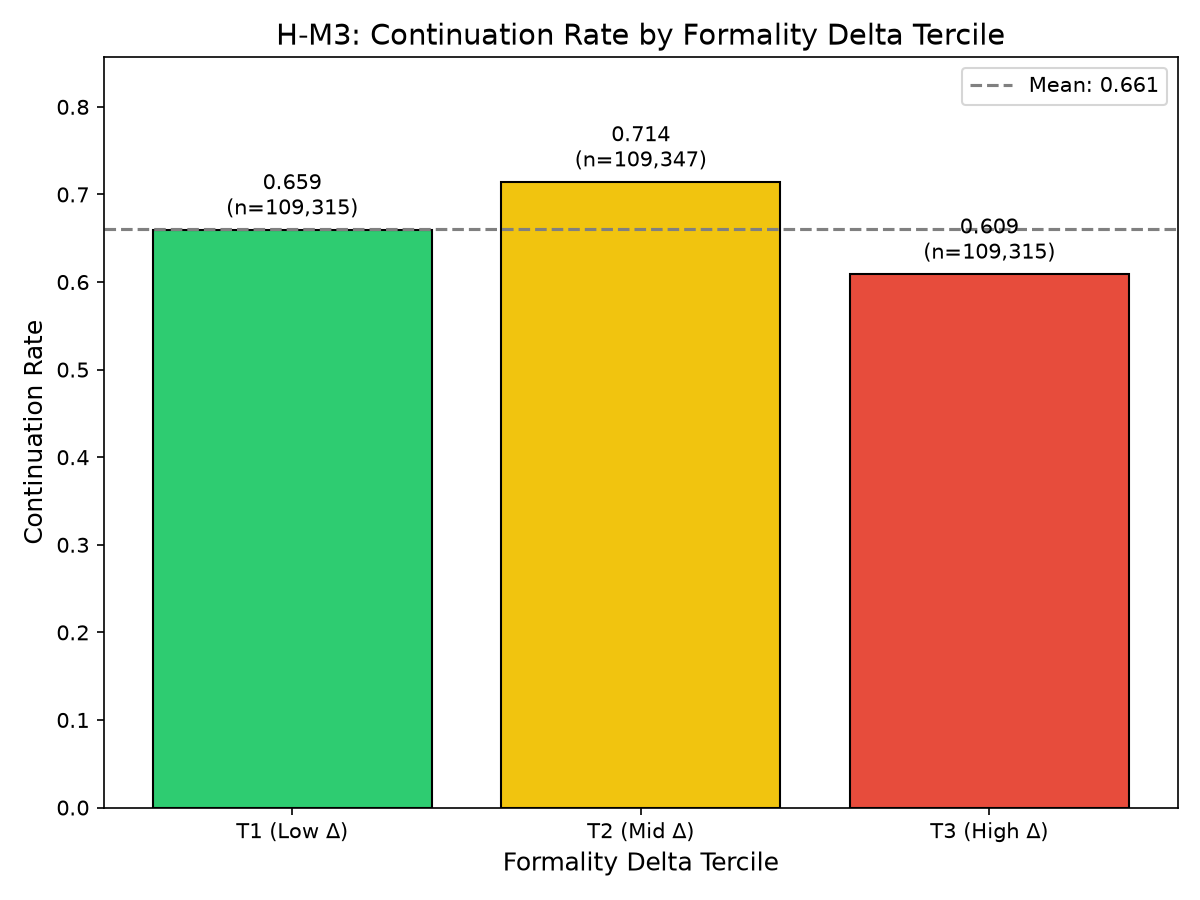
\includegraphics[width=\columnwidth]{figures/tercile_bar_chart.png}
\caption{Tercile continuation rates showing inverted-U pattern}
\label{fig:tercile_bar_chart}
\end{figure}

